\documentclass[12pt, a4paper]{article}

\usepackage{graphicx}


\title{Notulensi Pertemuan}
\author{BMKG 2}
\date{23 July 2022}

\begin{document}
\maketitle

\begin{tabbing}
\textbf{Hari/Tanggal}\quad\= Sabtu, 23 July 2022 \\
\textbf{Waktu} \>19.30 - 21.30 \\
\textbf{Tempat}\> Zoom Meeting
\end{tabbing}

Agenda pertemuan hari ini adalah:
\begin{enumerate}
\item pembuatan konten PPT
\item pembagian tugas presentasi
\item diskusi terkait mekanisme presentasi
\end{enumerate}

\bigskip 
Pada pertemuan kali ini, kami kembali berkumpul untuk mengerjakan konten PPT bersama dan membahas terkait adanya anggota kelompok yang seharusnya bertanggung jawab untuk membuat PPT dan video presentasi namun yang bersangkutan tidak bisa melanjutkan dalam tugas kelompok \emph{demo day} kali ini. PPT yang kelompok kami buat mengikuti \emph{template} dan bagian yang sudah ditentukan oleh panitia. Selain itu, kami juga membahas tentang pembagian tugas dalam presentasi sebagai berikut:
\begin{enumerate}
\item pembukaan dan pendahuluan oleh Risky Yoga Suratman
\item penjelasan \emph{data sets} dan LSTM oleh Taruma Sakti Megariansyah
\item penjelasan ANN oleh M Aldi
\item kesimpulan dan penutup oleh Krisna Malik Sukarno
\end{enumerate}

\medskip
Kami telah menyepakati \emph{virtual background} yang akan kami gunakan saat melakukan perekaman video presentasi. Hal ini bertujuan untuk membuat tampilan pada video presentasi akan lebih baik dan lebih rapih nantinya. Kami juga membahas tentang mekanisme dan manajemen waktu agar dapat memenuhi batas maksimal yang telah diberikan oleh panita yaitu 10 menit.


\bigskip
\section*{Dokumentasi}

\begin{figure}[h]
    \centering
    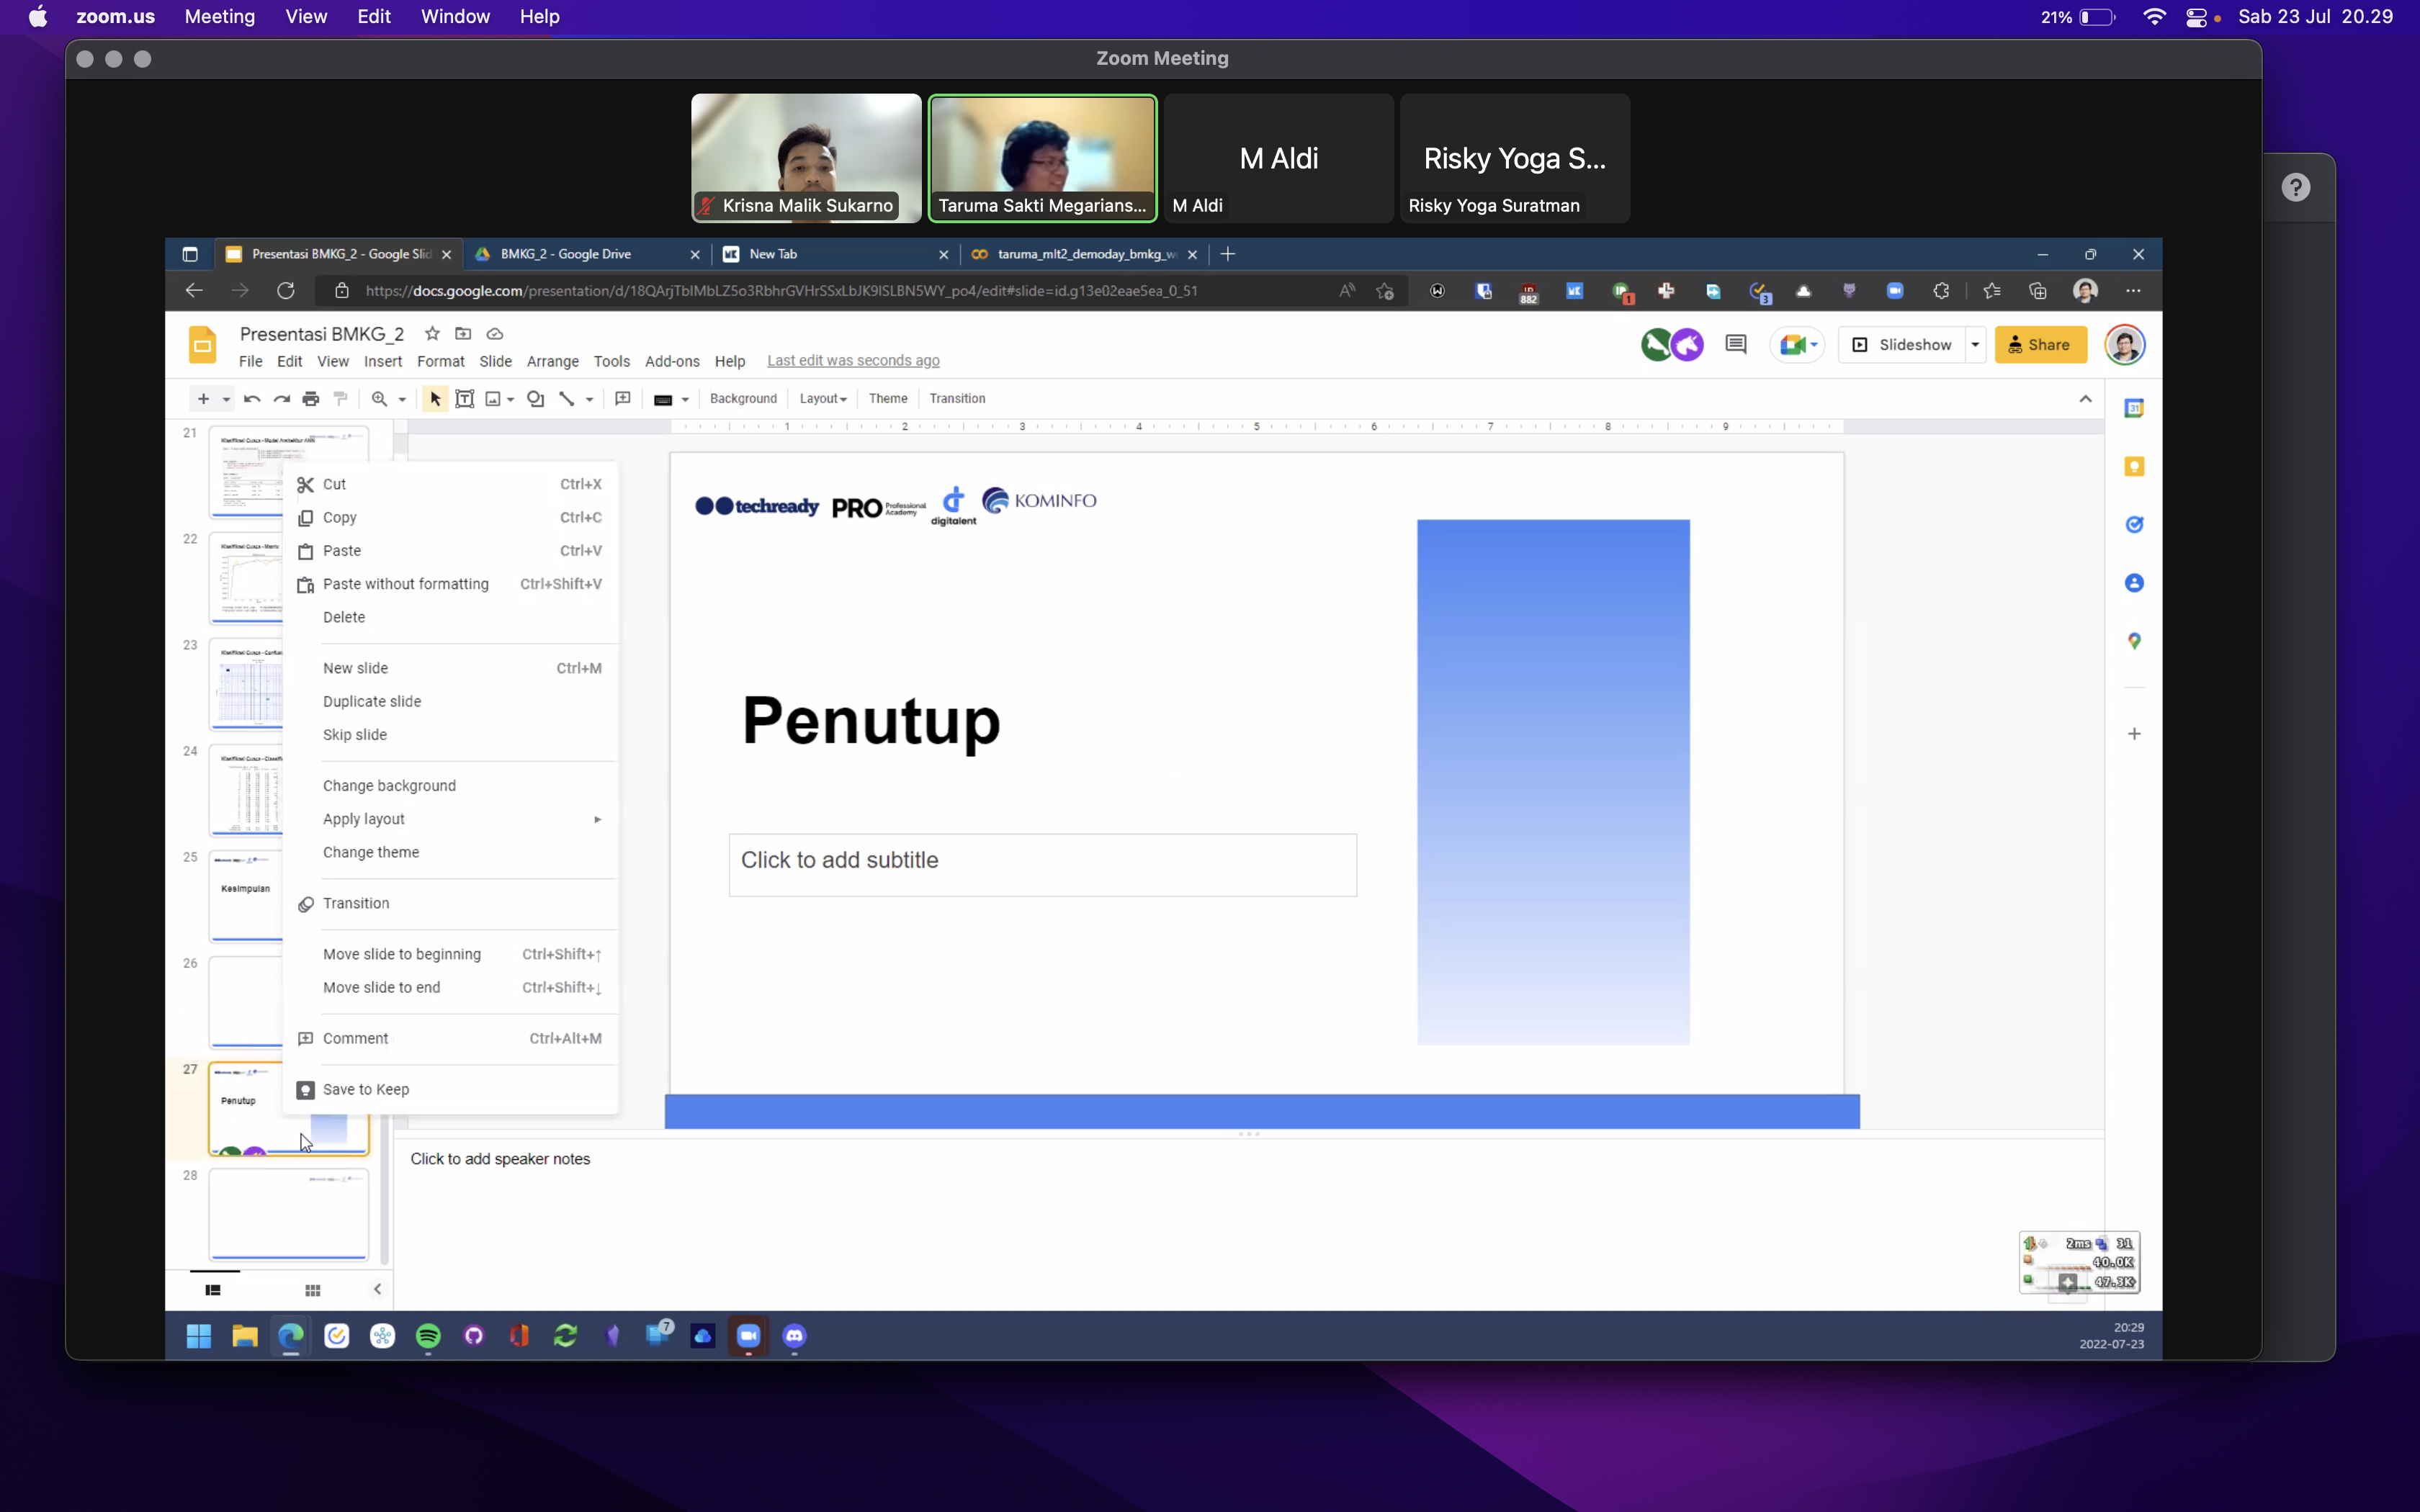
\includegraphics[width=\textwidth]{pert-3.1}
    \caption{Pembuatan Konten PPT}
\end{figure}

\begin{figure}[h]
    \centering
    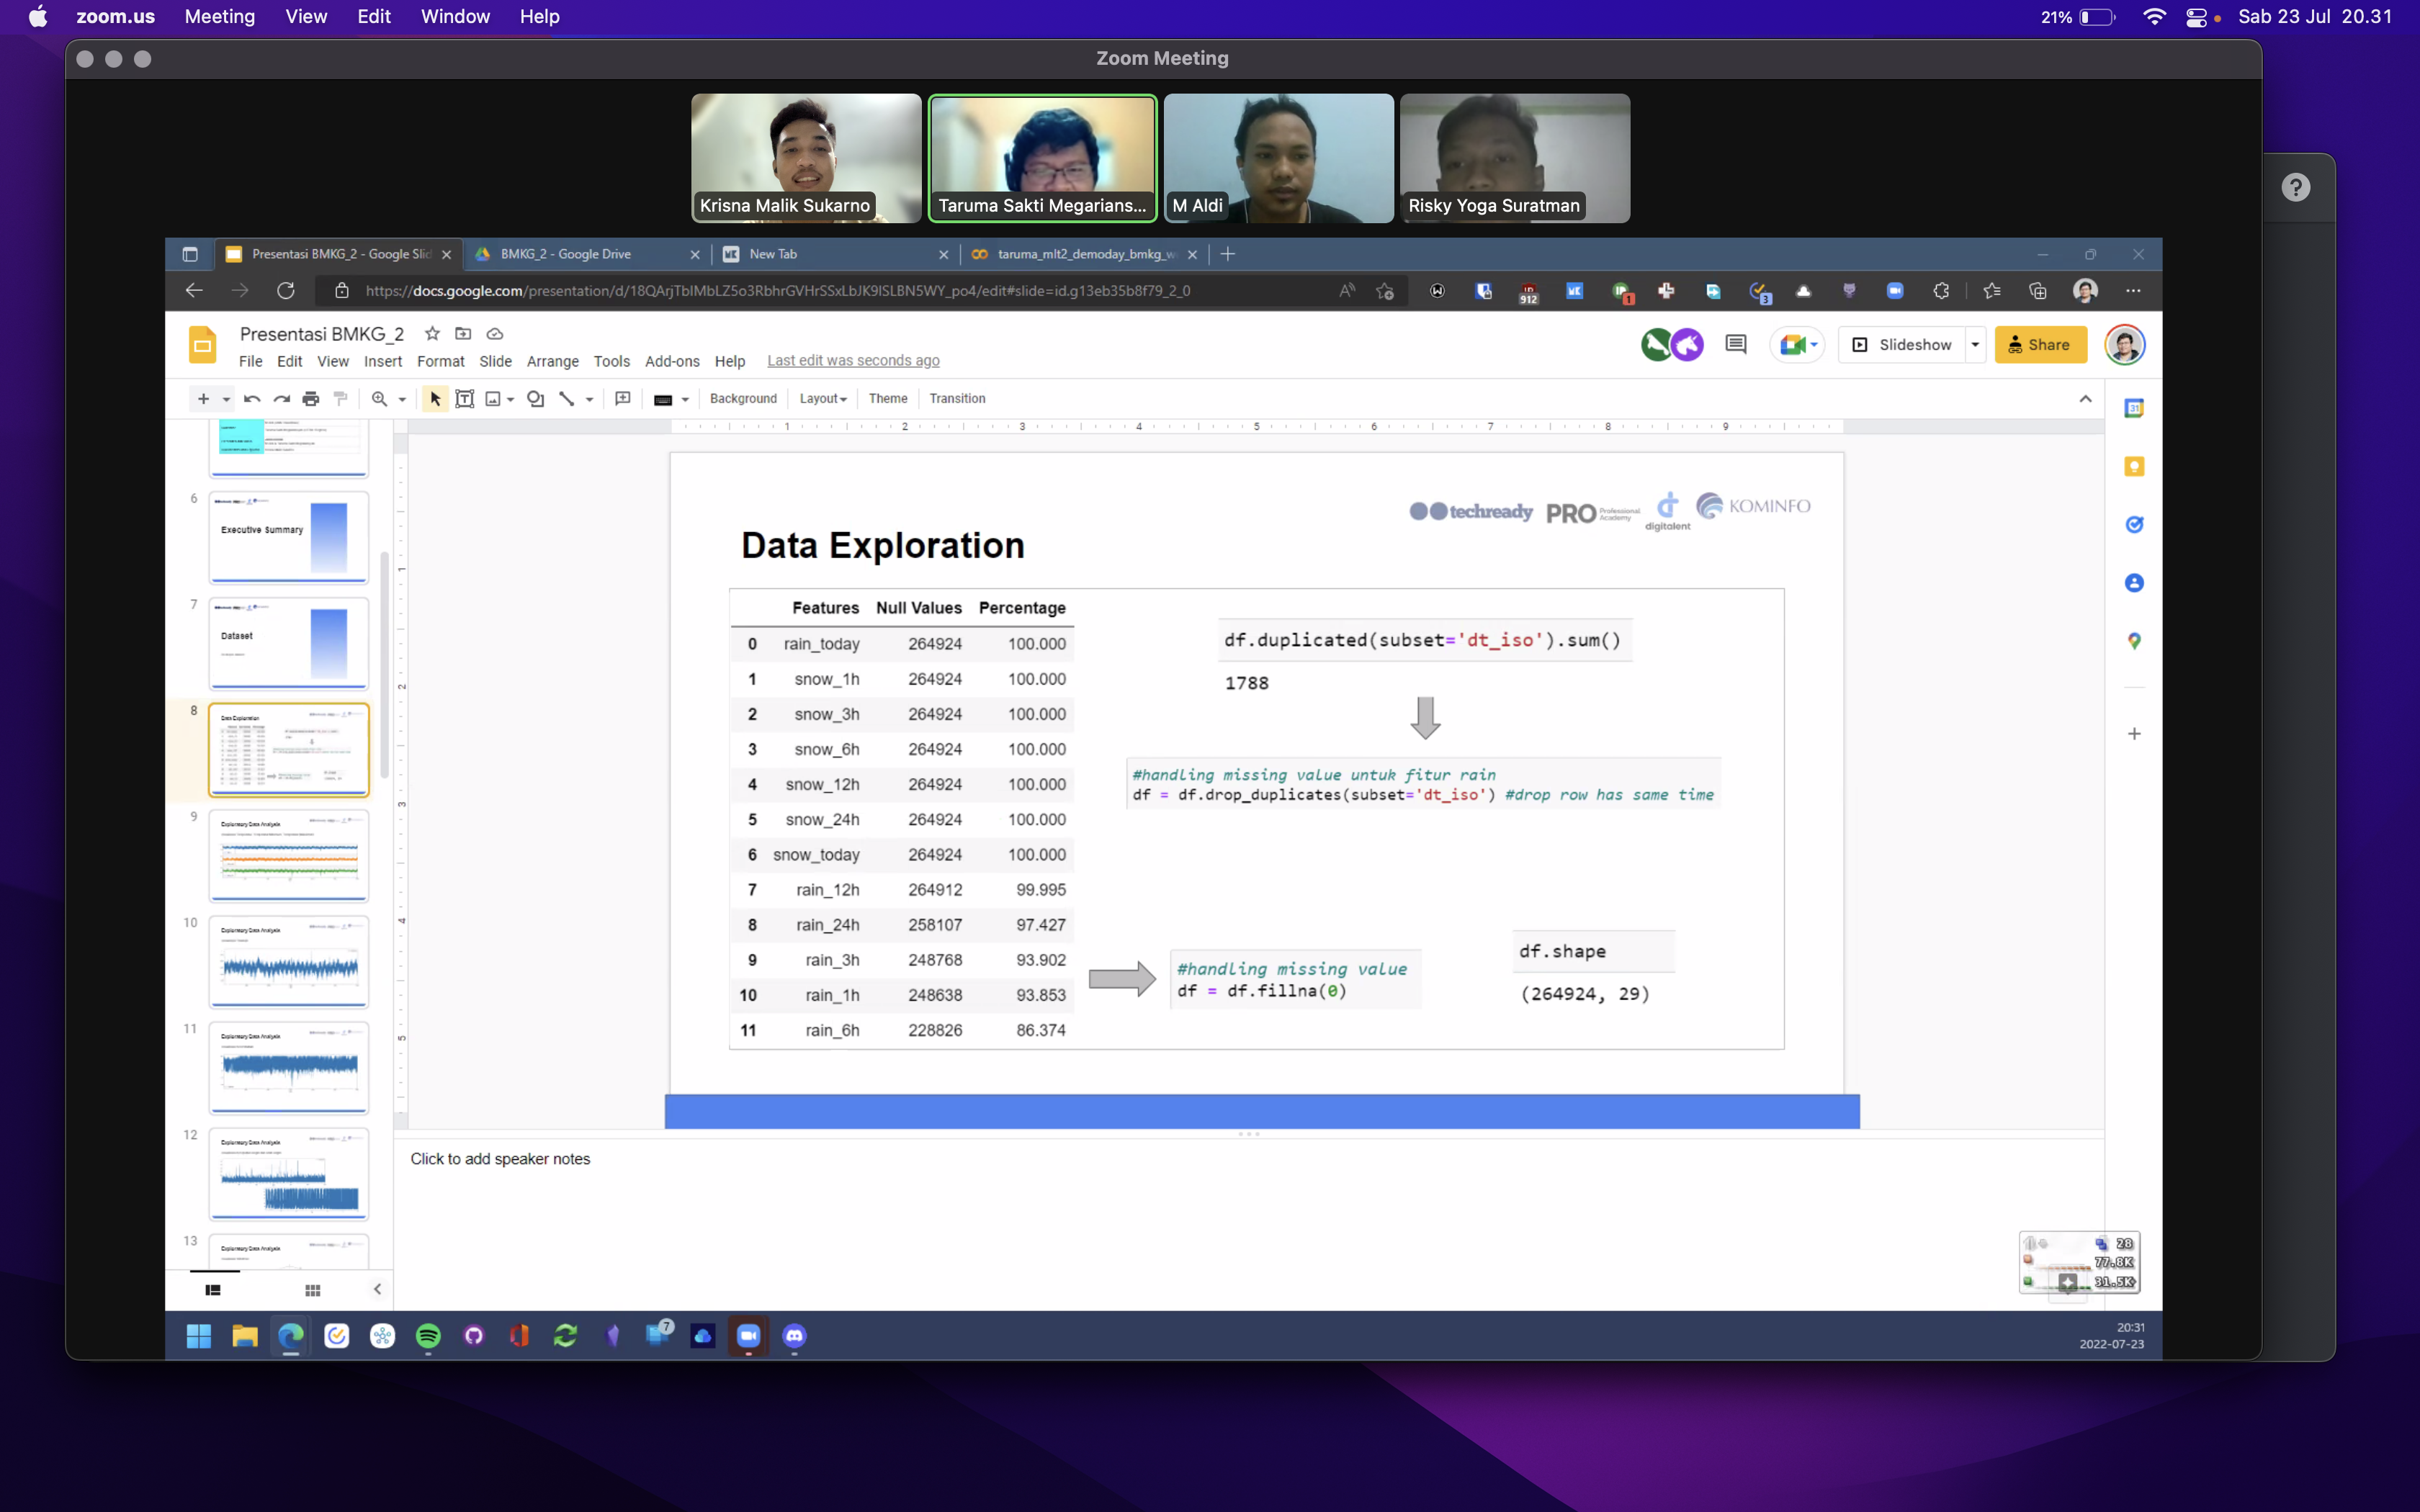
\includegraphics[width=\textwidth]{pert-3.2}
    \caption{Diskusi terkait mekanisme presentasi}
\end{figure}


\end{document}